The given transfer function can be expressed as
\begin{align}
    H(z) = \frac{16 - 6z^{-1}}{8 - 6z^{-1} + z^{-2}}\\
     = \frac{16 - 6z^{-1}}{(4 - z^{-1})(2 - {z^{-1}})}\\
      = \frac{4}{4 - z^{-1}} +\frac{2}{2 - z^{-1}}
%       = \frac{1}{1 - \frac{1}{4}z^{-1}} + \frac{1}{1 - \frac{1}{2}z^{-1}}
       \label{partial-fraction}
\end{align}
%
with poles at
\begin{align}
z = \frac{1}{2}, z = \frac{1}{4}
\end{align}
\begin{enumerate}
\item   Since the ROC includes the unit circle, the system is stable.  Also, the ROC extends outwards to infinity, so the system is causal as well.  Hence $S_1$ is true.
\item  When ROC = $\frac{1}{4} < \abs{z} < \frac{1}{2}$,  the unit circle is not included in the ROC.  Hence, the system cannot be stable.  Also, the ROC is an annulus, so the system is non-causal.  So $S_3$ is true.
\end{enumerate}
 

\begin{figure}[!ht]
\centering
 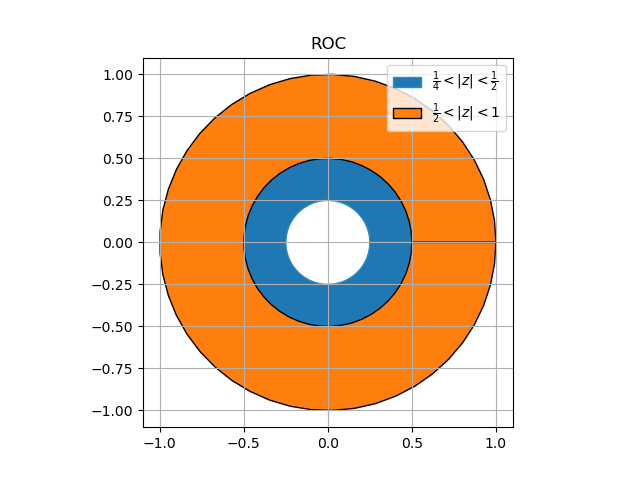
\includegraphics[width=\columnwidth]{solutions/ec/2010/42/Graphs/ROC.png}
 \caption{ROC}
 \end{figure}
 
 